% Settings for the default beamer theme
\documentclass[english, aspectratio=169]{beamer}
\usepackage[T1]{fontenc}
\usepackage[utf8]{inputenc}
\usepackage{tabularx}
\usepackage{babel}
\usepackage[ruled,vlined]{algorithm2e}
\SetAlgorithmName{Algoritmus}{algoritmus}{List of Algorithms}
\setcounter{secnumdepth}{3}
\setcounter{tocdepth}{3}

\makeatletter

\newcommand\makebeamertitle{\frame{\maketitle}}

% (ERT) argument for the TOC
\AtBeginDocument{%
  \let\origtableofcontents=\tableofcontents
  \def\tableofcontents{\@ifnextchar[{\origtableofcontents}{\gobbletableofcontents}}
  \def\gobbletableofcontents#1{\origtableofcontents}
}

% Theme settings
\usetheme{Frankfurt}
\usecolortheme{default}
\usefonttheme[onlymath]{serif}

% Template settings
\setbeamertemplate{navigation symbols}{}
\setbeamertemplate{blocks}[rounded][shadow=false]
\setbeamertemplate{title page}[default][colsep=-4bp, rounded=true, shadow=false]
\makeatother

% Define a custom darker red color
\definecolor{DarkerRed}{RGB}{139,0,0} % Adjust the RGB values as needed

% Use the newly defined color in Beamer theme elements
\setbeamercolor{structure}{fg=DarkerRed} % Changes basic structural elements to Darker Red
\setbeamercolor{title in head/foot}{bg=DarkerRed} % Changes the title in header/footer to Darker Red


\begin{document}

% Title page
\section{Bevezetés}
\title[]{Üzleti Elemzések Módszertana}
\subtitle{11. Előadás: Megerősítéses tanulás}
\author[Kuknyó Dániel]{Kuknyó Dániel\\Budapesti Gazdasági Egyetem}
\date{2023/24\\2.félév}
\makebeamertitle

% Table of contents slide
\begin{frame}
\tableofcontents{}
\end{frame}

% Table of contents of the current section
\begin{frame}
\tableofcontents[currentsection]
\end{frame}

\begin{frame}{A gépi tanulás fajtái}
A gépi tanulás 3 fő irányzata:
\begin{itemize}
	\item Felügyelt tanulás
	\item Felügyelet nélküli tanulás
	\item Megerősítéses tanulás
\end{itemize}
\begin{center}

\includegraphics[width=12cm, height=7cm, keepaspectratio]{images/reinforcement_1.png}
\end{center}
\end{frame}

\begin{frame}{Mikor alkalmazható a megerősítéses tanulás?}
\begin{columns}
\begin{column}{.5\textwidth}
Az RL olyan problémák esetén használatos, ahol\textbf{ az algoritmikus vagy hagyományos ML hozzáállás nem bizonyul megfelelőnek}, mert nem lehetséges tanító adatot gyűjteni vagy generálni.\par\smallskip
Például:
\begin{itemize}
	\item Robotok
	\item Autonóm vezetés
	\item Számítógépes játékok
\end{itemize}
\end{column}
\begin{column}{.5\textwidth}
\begin{center}
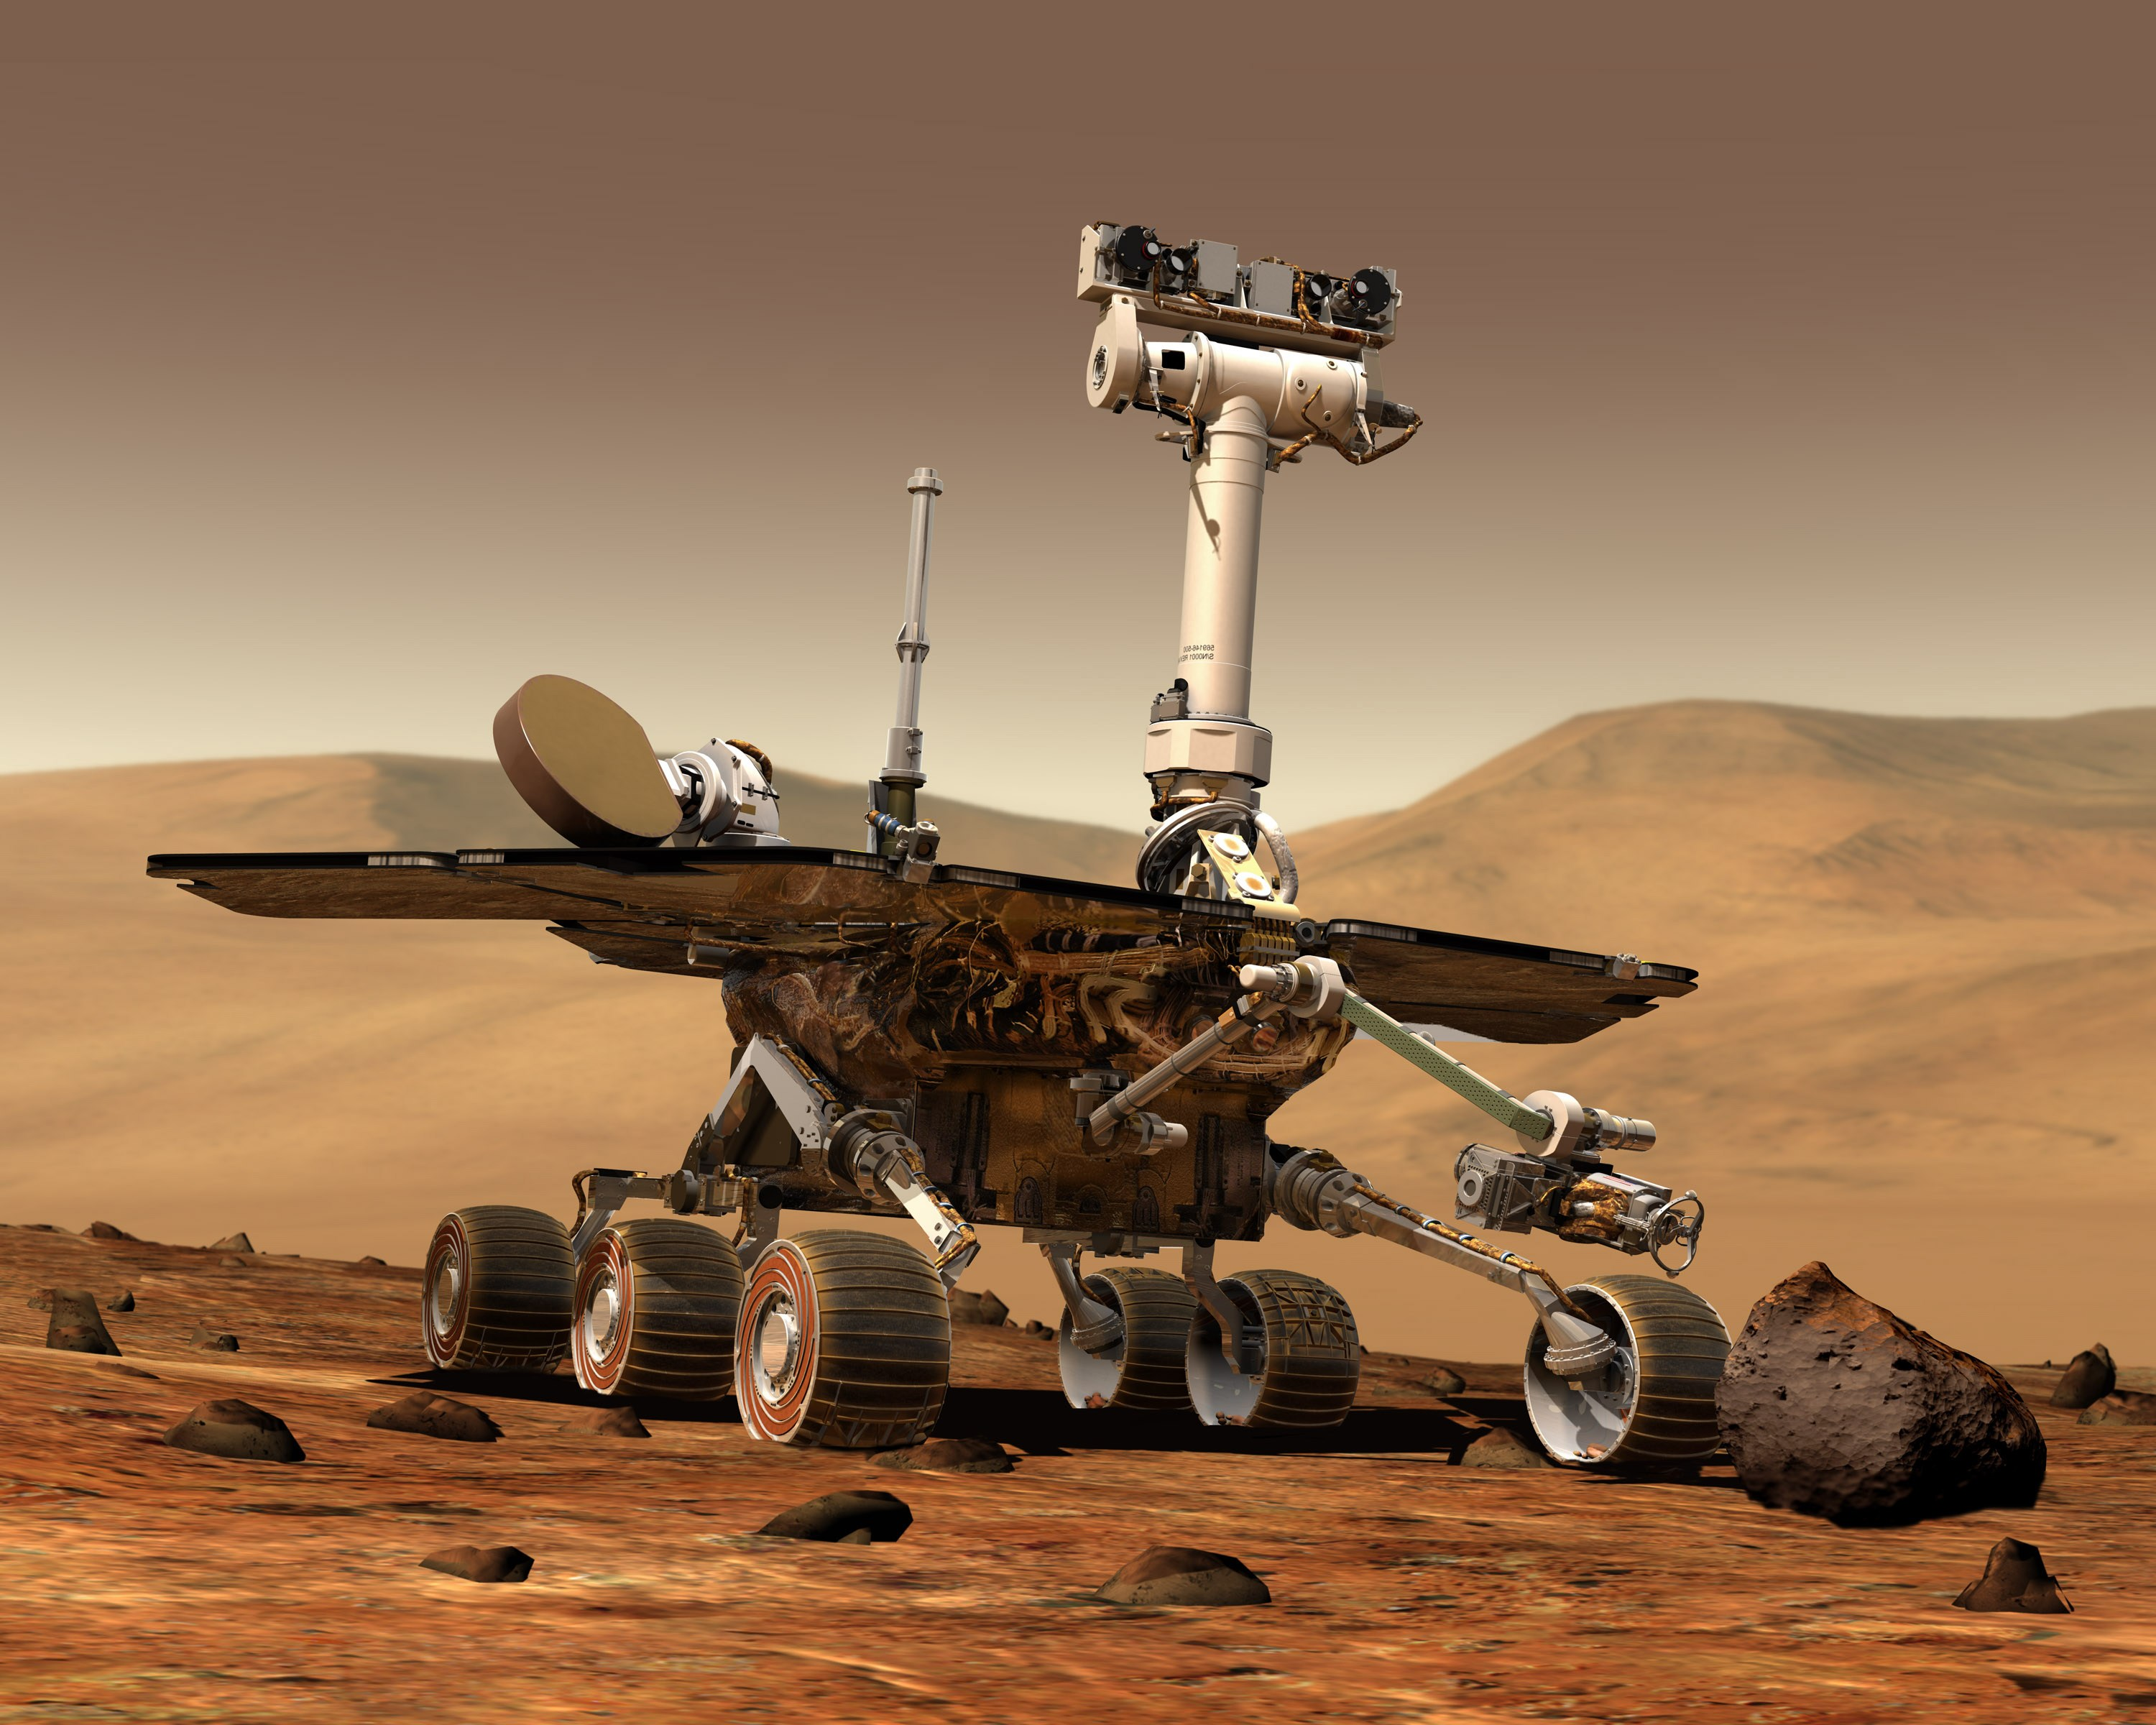
\includegraphics[width=3cm, height=2.5cm]{images/reinforcement_2.png}
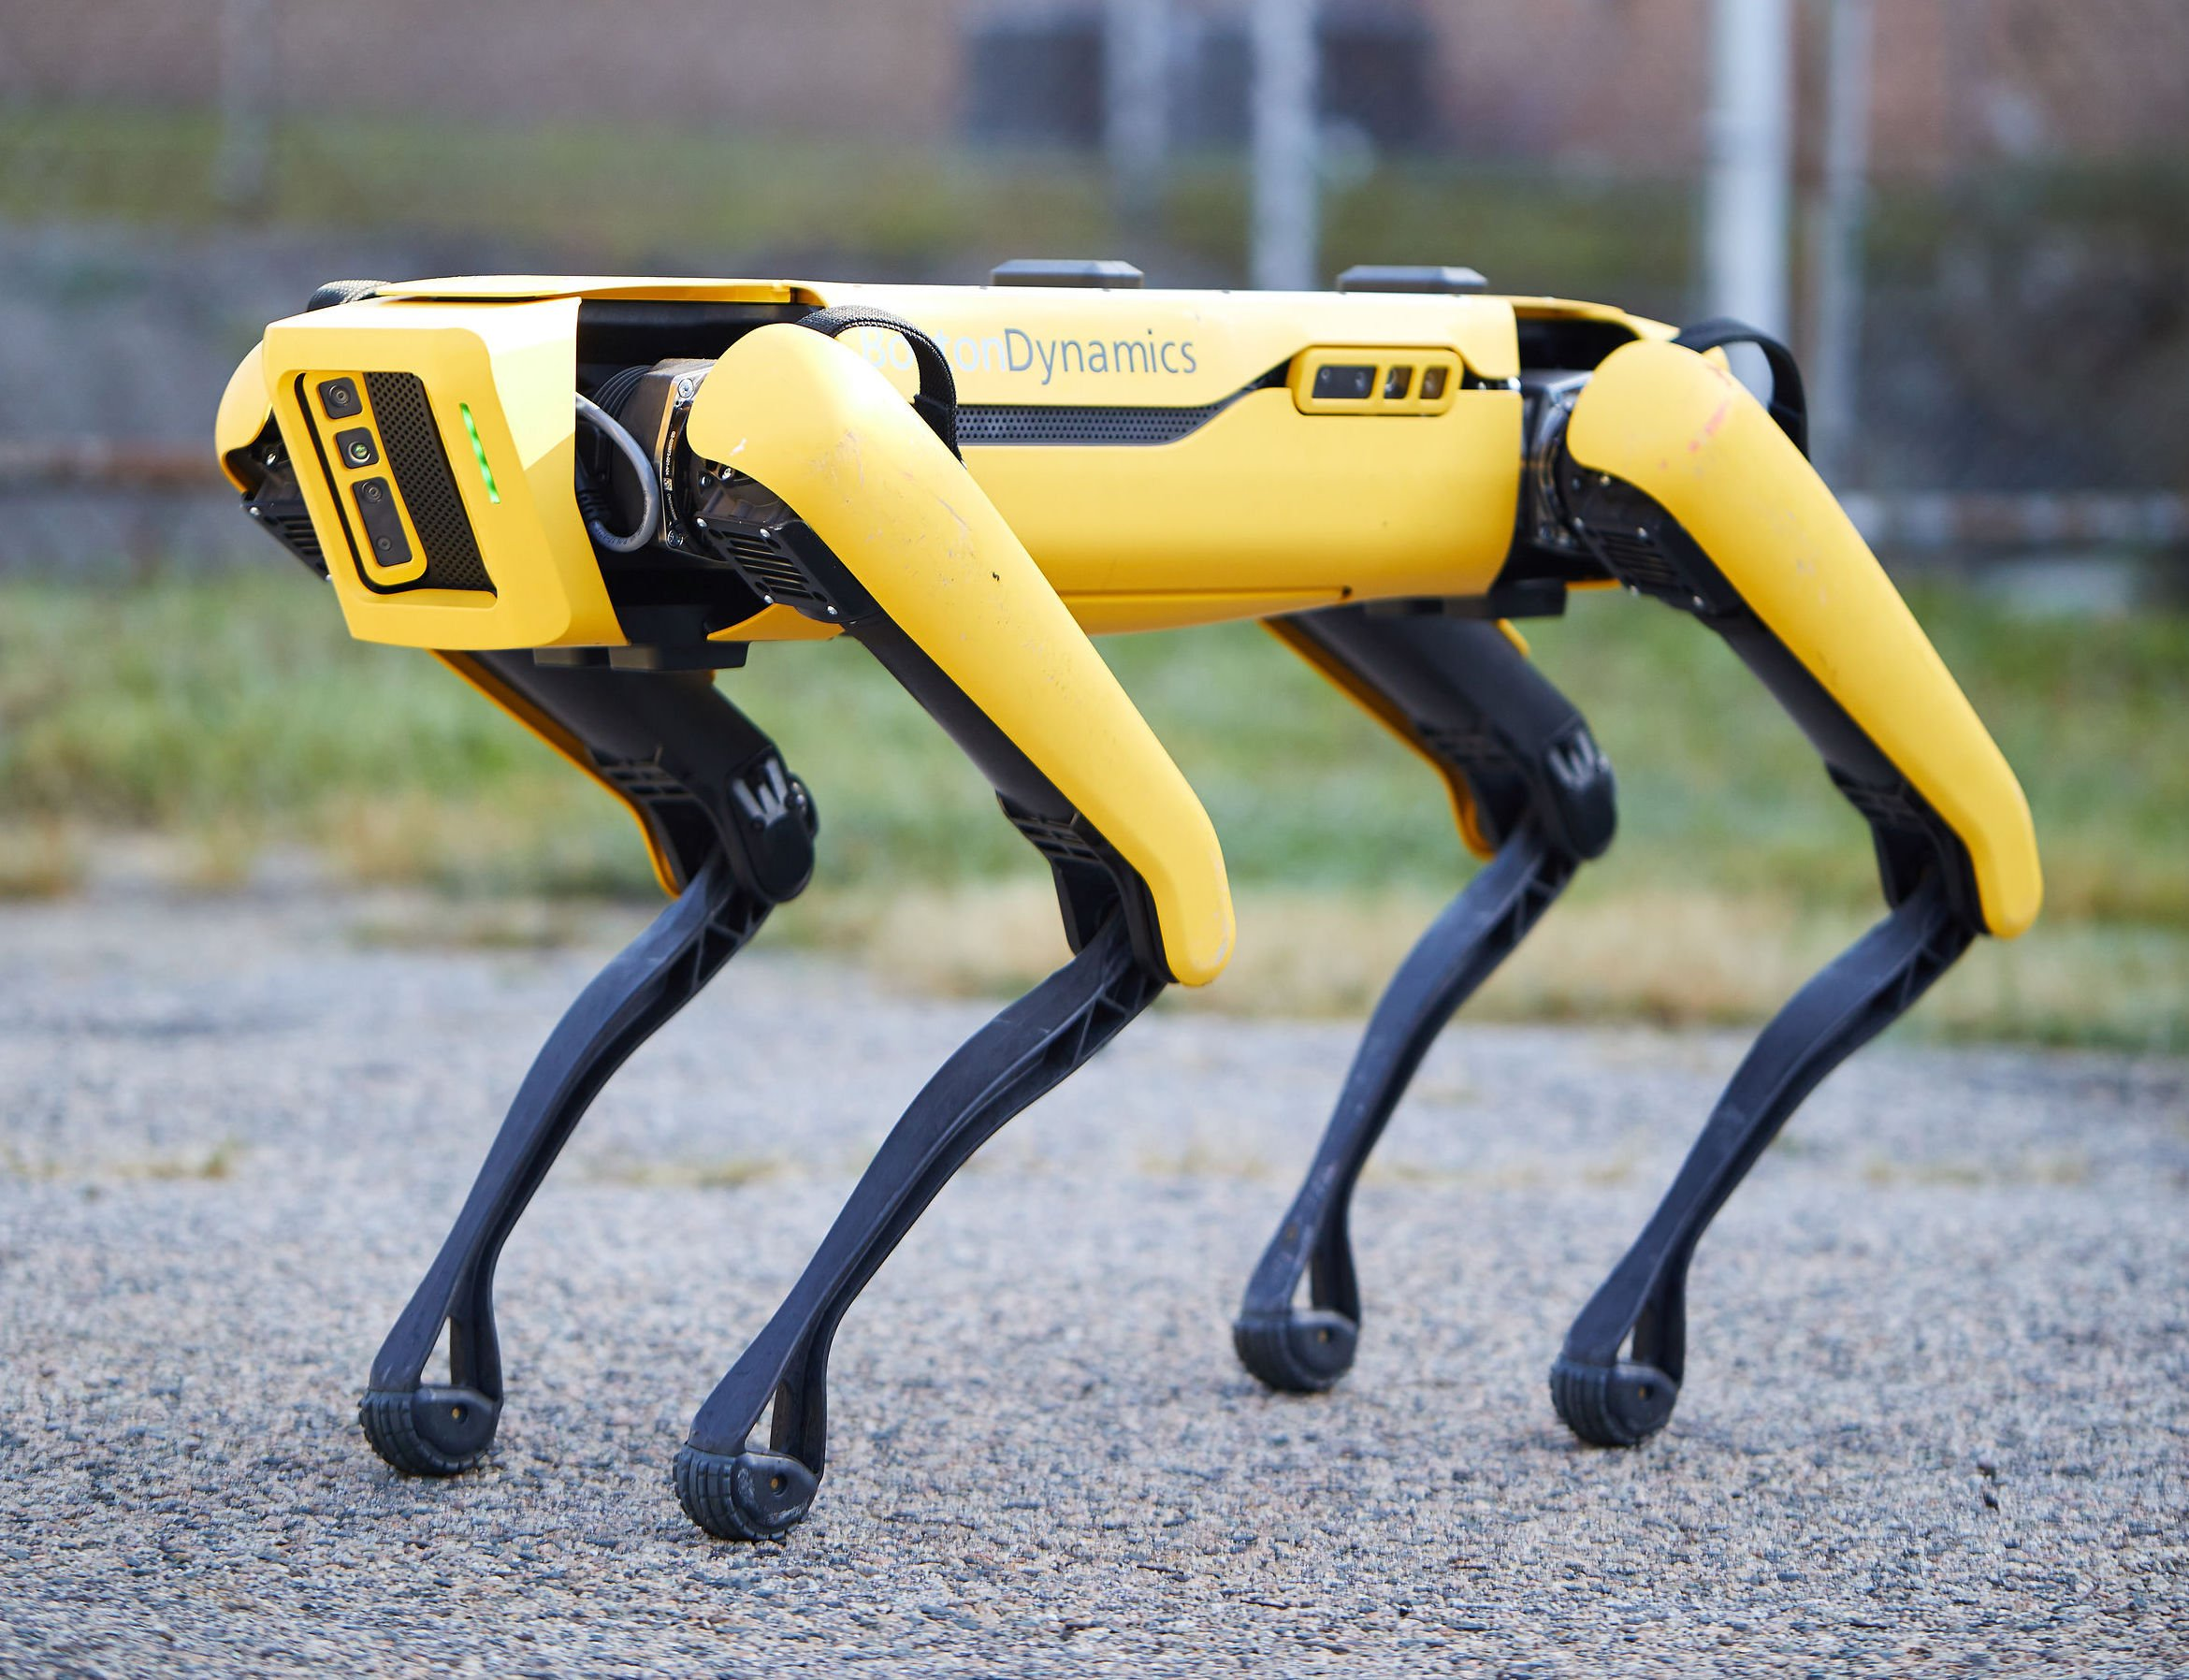
\includegraphics[width=3cm, height=2.5cm]{images/reinforcement_3.png}
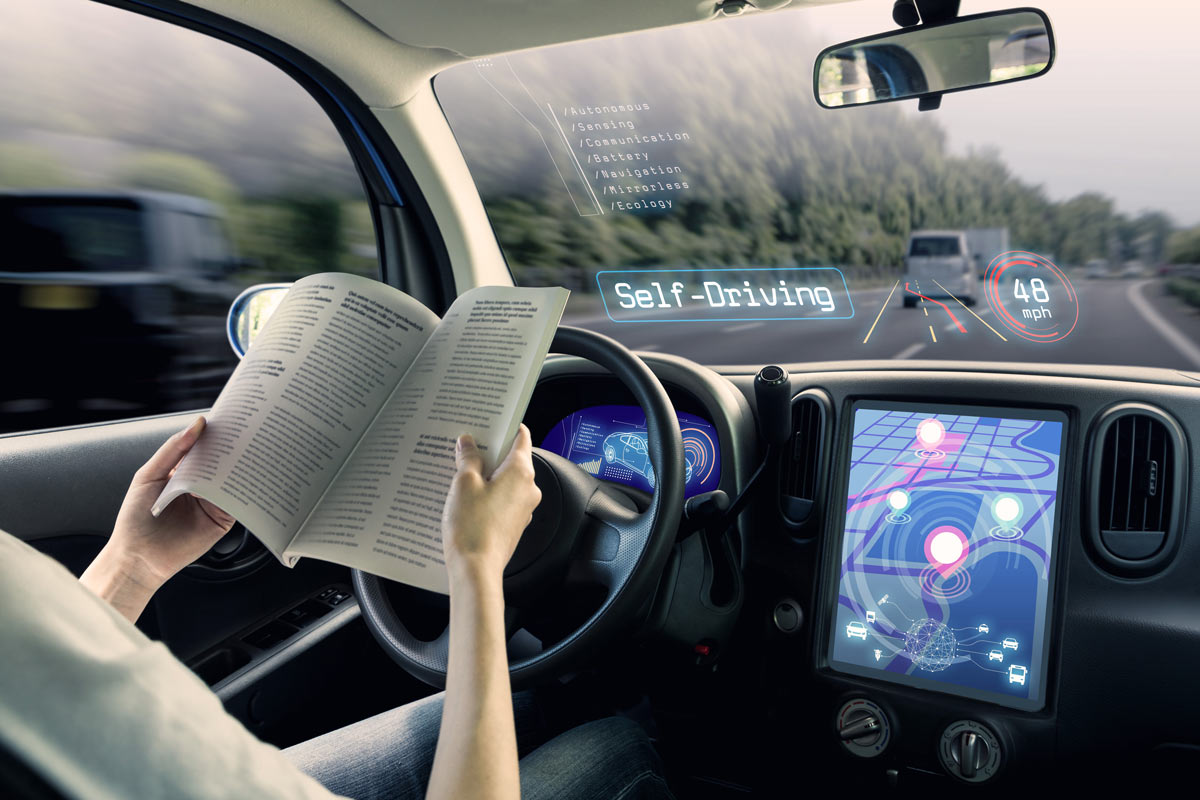
\includegraphics[width=3cm, height=2.5cm]{images/reinforcement_4.png}
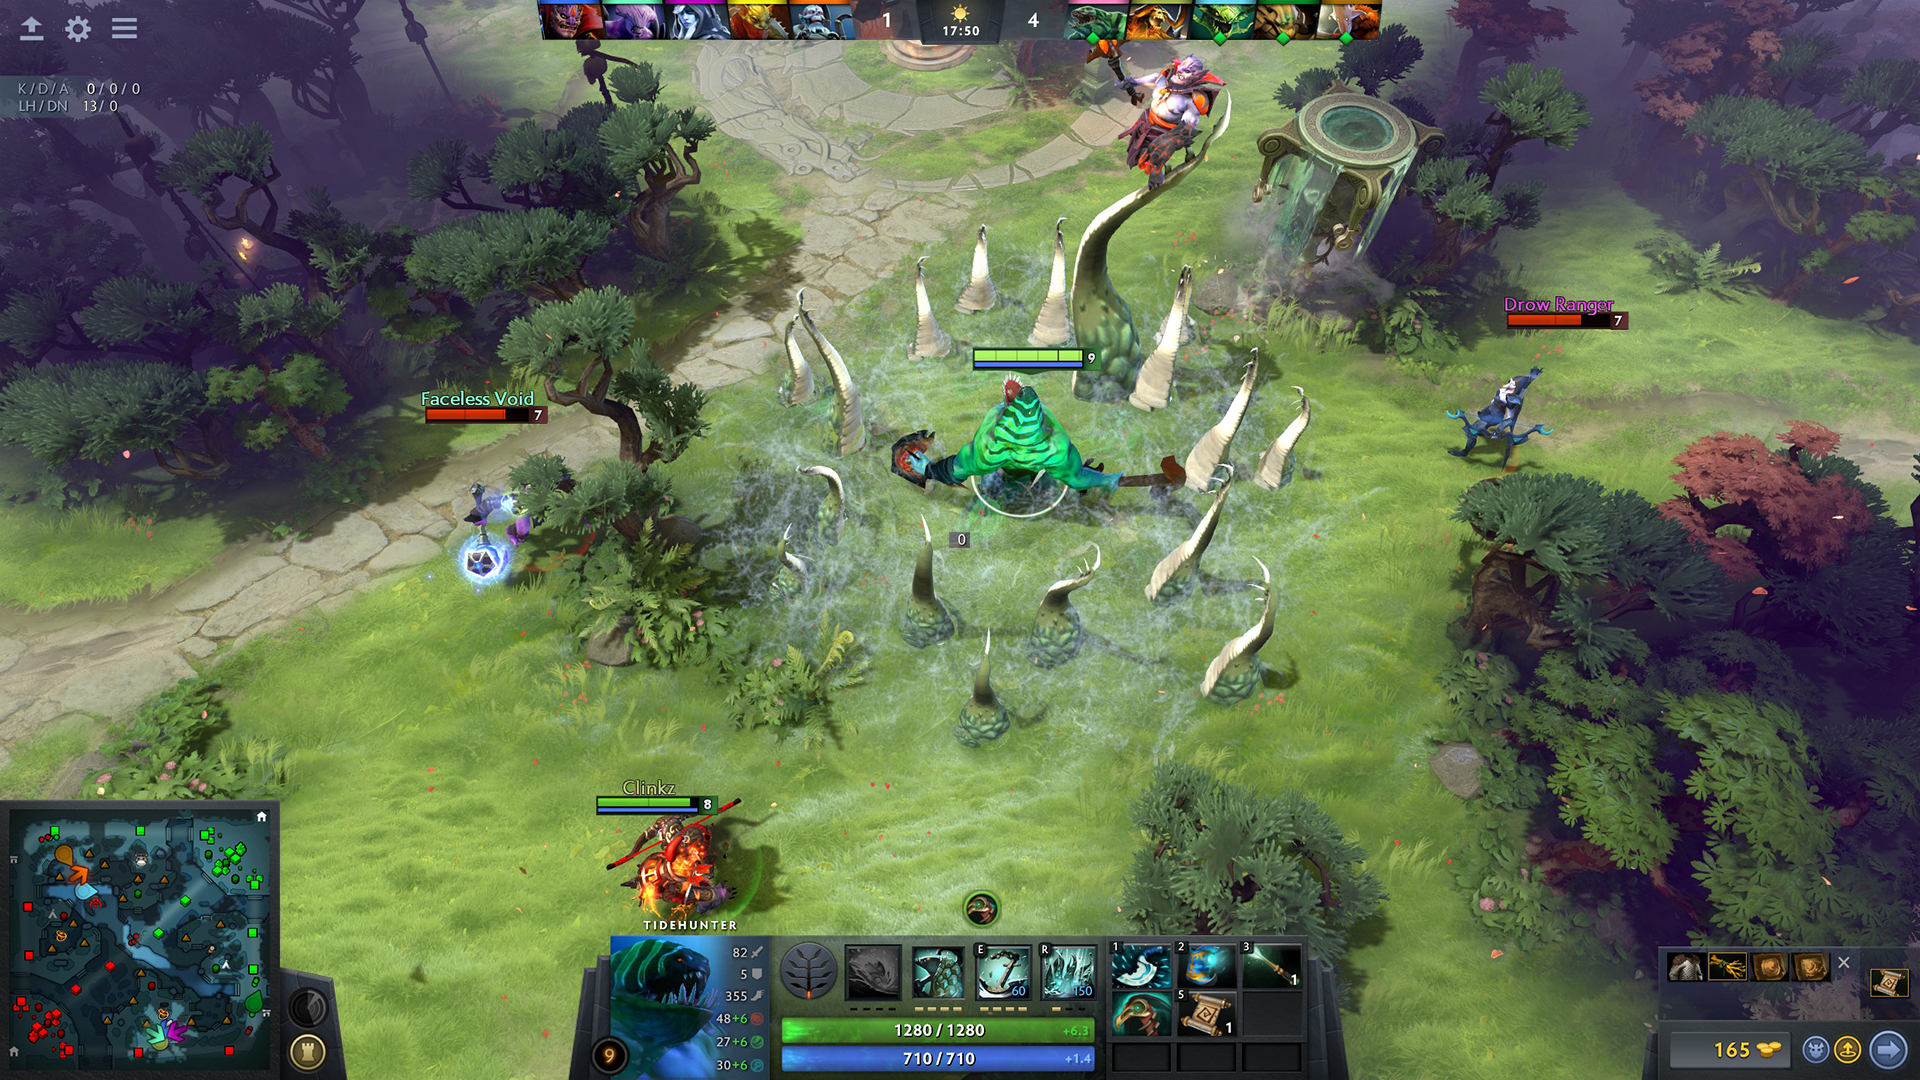
\includegraphics[width=3cm, height=2.5cm]{images/reinforcement_5.png}
\end{center}
\end{column}
\end{columns}
\end{frame}

\begin{frame}{Felügyelt vagy megerősítéses tanulás?}
\begin{columns}
\begin{column}{.5\textwidth}
Adott például egy autóversenyző program. Ha felügyelt tanítás a választott hozzáállás, \textbf{szükség van egy adatbázisra, amely jellemzi az összes szituációt, és minden szituációhoz tartozóan az elvárt output értéket}.\par\medskip
A szituációknak le kell írnia a kocsi helyzetét, a környezet állapotát, a versenytársak helyzetét. Az elvárt outputnak olyan halmazból kell kikerülnie, mint gáz, jobb, bal, fék és ezek kombinációi.
\end{column}
\begin{column}{.5\textwidth}
\begin{center}
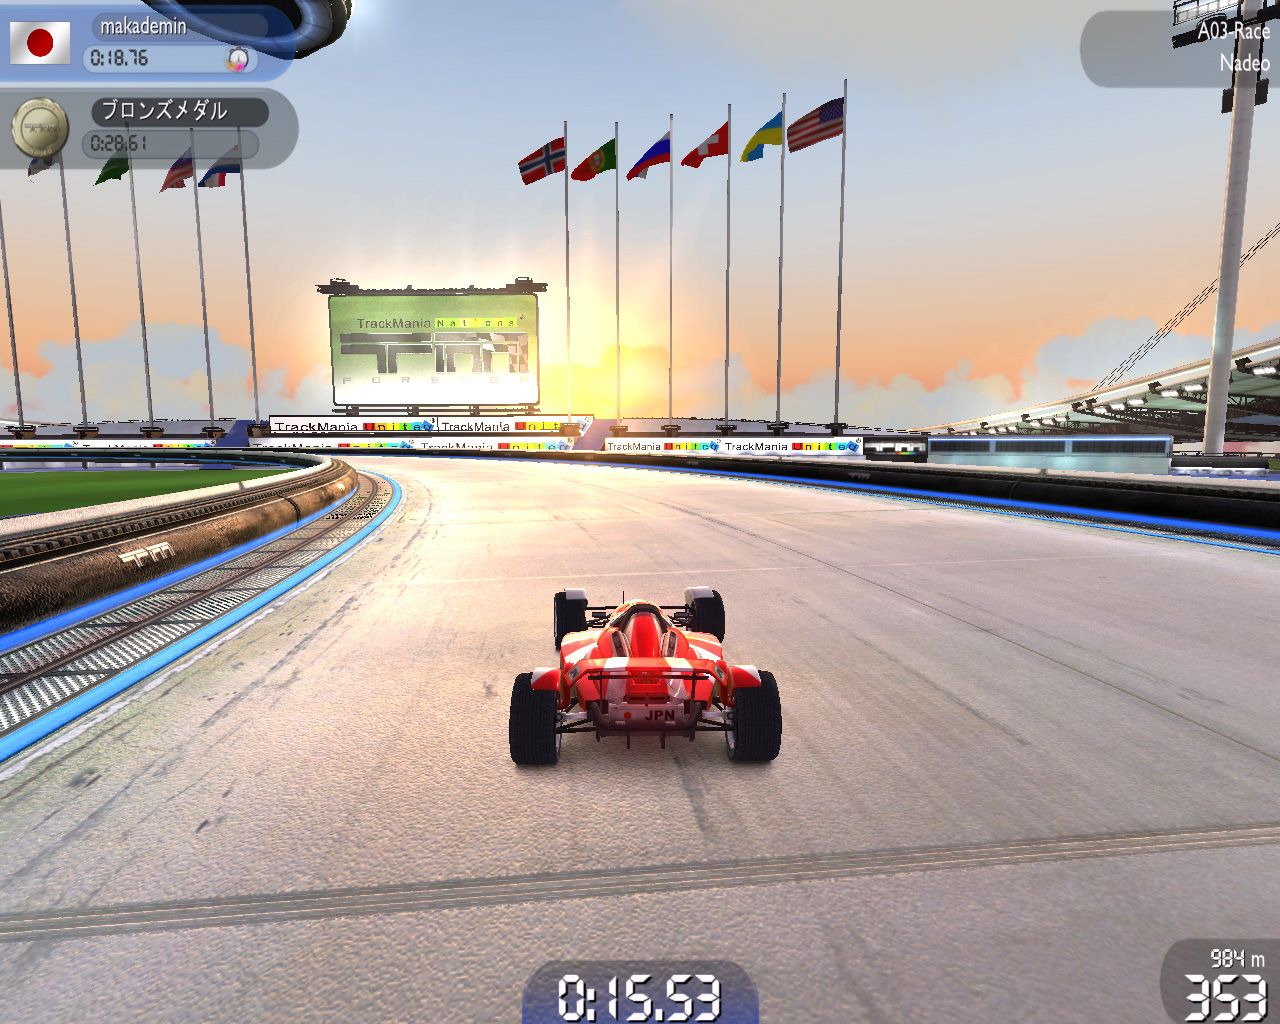
\includegraphics[width=6cm, height=7cm, keepaspectratio]{images/reinforcement_6.png}
\end{center}
\end{column}
\end{columns}
\end{frame}

\begin{frame}{Visszajelzések a megerősítéses tanulásban}
\begin{columns}
\begin{column}{.5\textwidth}
A két szemléletmód abban különbözik, hogy a felügyelő milyen visszajelzéseket ad a tanulónak.\par\medskip
\only<1>{\textbf{A felügyelt tanulásban teljes visszajelzésekről van szó, mert a válasz önmagában a  megoldás.}}
\only<2>{\textbf{A megerősítéses tanulásban viszont csak részlegesek a visszajelzések. A felügyelő válasza mindig csak a megoldás irányába vezet, nem önmagában a teljes jó megoldás.}}
\end{column}
\begin{column}{.5\textwidth}
\begin{center}
\includegraphics<1>[width=7cm, height=7cm, keepaspectratio]{graphs/reinforcement_1.png}
\includegraphics<2>[width=7cm, height=7cm, keepaspectratio]{graphs/reinforcement_2.png}
\end{center}
\end{column}
\end{columns}
\end{frame}

\end{document}
















